% Exact spectral regions and schematic locations; no numerical spectrum is plotted.
% Requires only tikz and the manuscript's standard mathematical packages.
\begin{figure}[tbp]
\centering
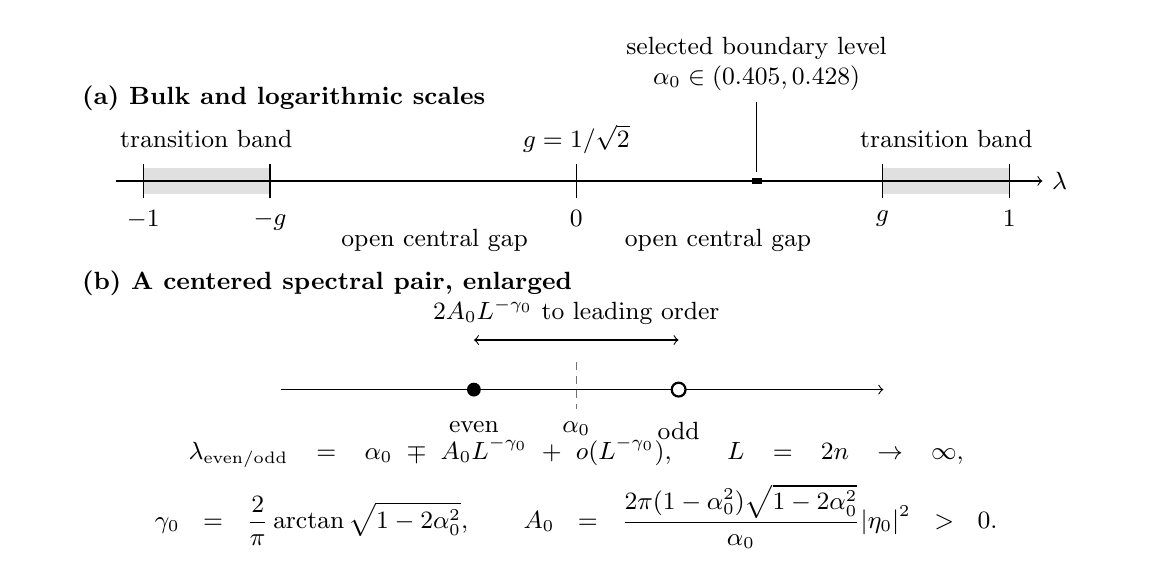
\begin{tikzpicture}[x=1cm,y=1cm,font=\small]
  \node[anchor=west,font=\small\bfseries] at (-6.4,1.05)
    {(a) Bulk and logarithmic scales};
  \fill[black!12] (-5.5,-0.16) rectangle (-3.889,0.16);
  \fill[black!12] (3.889,-0.16) rectangle (5.5,0.16);
  \draw[->] (-5.85,0) -- (5.92,0) node[right] {$\lambda$};
  \foreach \x/\lab in {-5.5/{-1},-3.889/{-g},0/{0},3.889/{g},5.5/{1}} {
    \draw (\x,-0.22) -- (\x,0.22);
    \node[anchor=north] at (\x,-0.25) {$\lab$};
  }
  \node at (-4.7,0.53) {transition band};
  \node at (4.7,0.53) {transition band};
  \node at (0,0.53) {$g=1/\sqrt2$};
  \node at (-1.8,-0.75) {open central gap};
  \node at (1.8,-0.75) {open central gap};
  \draw[line width=2pt] (2.2275,0) -- (2.354,0);
  \draw (2.29,0.12) -- (2.29,1.00);
  \node[anchor=south,align=center] at (2.29,1.02)
    {selected boundary level\\$\alpha_0\in(0.405,0.428)$};
  \node[anchor=west,font=\small\bfseries] at (-6.4,-1.30)
    {(b) A centered spectral pair, enlarged};
  \draw[->] (-3.75,-2.65) -- (3.9,-2.65);
  \draw[densely dashed,black!55] (0,-2.30) -- (0,-2.90);
  \node[anchor=north] at (0,-2.94) {$\alpha_0$};
  \fill (-1.30,-2.65) circle (2.5pt);
  \draw[fill=white,line width=0.8pt] (1.30,-2.65) circle (2.5pt);
  \node[anchor=north] at (-1.30,-2.94) {even};
  \node[anchor=north] at (1.30,-2.94) {odd};
  \draw[<->] (-1.30,-2.02) -- (1.30,-2.02);
  \node[anchor=south] at (0,-1.95) {$2A_0L^{-\gamma_0}$ to leading order};
  \node[align=center,text width=13.7cm] at (0,-3.96) {
    $\displaystyle
    \lambda_{\mathrm{even/odd}}
       =\alpha_0\mp A_0L^{-\gamma_0}+o(L^{-\gamma_0}),\qquad L=2n\to\infty,$\\[5pt]
    $\displaystyle
    \gamma_0=\frac2\pi\arctan\sqrt{1-2\alpha_0^2},\qquad
    A_0=\frac{2\pi(1-\alpha_0^2)\sqrt{1-2\alpha_0^2}}{\alpha_0}
          |\eta_0|^2>0.$};
\end{tikzpicture}
\caption{Spectral scales for the single-frequency operator.
The shaded bands support the logarithmic trace density, whereas the
bulk values are $\pm1$. The marked interval encloses the certified
phase-zero half-line level; it is not a census of the central gaps.
The enlarged panel shows the leading locations of the two eigenvalues
of $\mathcal K_n$ converging to that level. Their placement is schematic,
not numerical data. Here $\eta_0$ is the normalized physical tail
amplitude. The coefficient includes the complementary-resolvent
contribution, and $|\eta_0|>1/100$ makes it nonzero.}
\label{fig:unified-spectral-roadmap}
\end{figure}
